\begin{figure*}
    \centering
    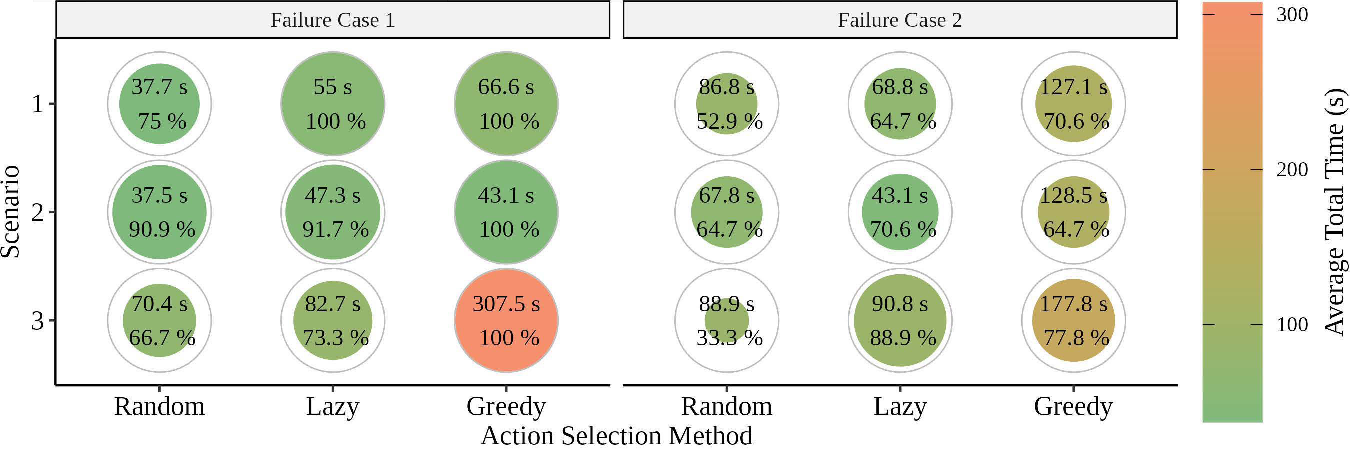
\includegraphics[width=\textwidth]{figures/both_flipped_5.pdf}
    \caption{Comparative performance of Action Selection Methods across the Failure Cases. The color intensity of each circle indicates the task time, with green colors representing lower times and red colors indicating higher times. The size of each circle represents the success rate, with larger circles denoting higher rates.\vspace{-10pt}}
    \label{fig:bubble}
\end{figure*}
\begin{figure*}
    \centering
    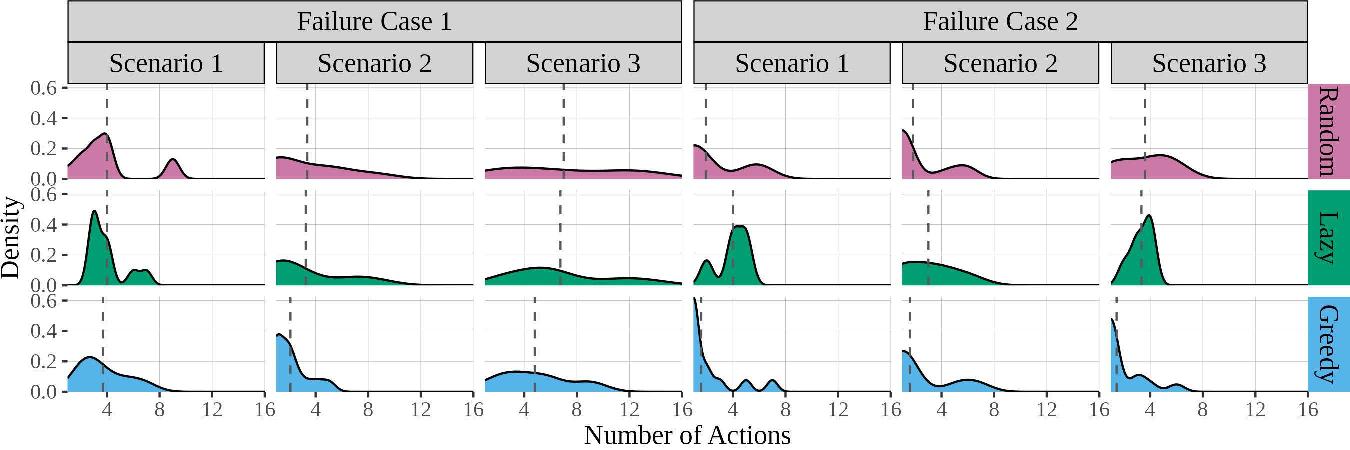
\includegraphics[width=\textwidth]{figures/shoulder_wrist_actions_comp_3.pdf}
    \caption{The distribution of actions required to complete different scenarios for each failure case using the action selection methods. Each graph represents a scenario under a specific failure case, with the x-axis indicating the number of actions and the y-axis representing the density across all trials. \vspace{-10pt}}
    \label{fig:shoulder-actions-comp}
\end{figure*}
\subsection{Real-world Manipulation Results}\label{sec:planner_eval}
% \begin{table}[]
% \centering
% \begin{tabular}{ccccc}
% \hline
% \textbf{}       & \multicolumn{3}{c}{\textbf{Task Time {[}seconds{]}}}                        & \textbf{Success Rate} \\ \hline
% \textbf{Planner}  & \textbf{S1} & \textbf{S2} & \textbf{S3} & \textbf{S1-S3} \\
% \textbf{Lazy} & \textit{\textbf{69.53}} & \textit{\textbf{62.25}} & \textit{\textbf{85.92}} &\textit{ \textbf{75.0\%}}       \\
% \textbf{greedy} & 146.23      & 130.46      & 127.53      & 61.2\%         \\
% \textbf{Random}   & 97.37       & 74.26       & 94.64       & 60.0\%         \\ \hline
% \end{tabular}
% \caption{Task Times For Failure Case 2}
% \label{tab:task-times-fc2}
% \end{table}


\cref{fig:bubble} shows the average total task time and success rates across Scenarios 1-3, Failure Cases 1 and 2, and the Random, Lazy, and Greedy ASMs. Across the ASMs, we see a trend of the Greedy method taking the longest, up to 307.5s, and the Random method taking the shortest time, as low as 37.5s, to complete the task, with the Lazy method roughly falling in between, at 47.3s-82.7s. This is expected because when averaged over all scenarios, the Greedy edge selection takes more time to plan than the other methods. Regarding the success rate, we see a clear trend in Failure Case 1, where the Greedy edge selection method has a 100\% success rate across all scenarios, and the Random edge selection has the lowest success rate. The Lazy edge selection has a success rate that, at best, matches the Greedy selection method at 100\% and, at worst, is better than the Random selection method, at 73.3\% vs. 66.7\% for Scenario 3. However, for Failure Case 2, no clear trend for the success rate occurs. Overall, the Lazy selection case is successful in scenarios 2 and 3, while the other two ASMs tend to have poorer results, except in scenario 1 for the Greedy ASM at 70.6\%. These results come from the combination of the inherent stochastic nature of the NPM interactions multiplied by the decreased sim-to-real accuracy of our sim-in-the-loop planner when interacting with areas of the robot that are not the end effector, as this failure case requires. This can partly be explained by the slight differences between our simulated collision meshes and the real robot embodiment.

% \begin{table}[]
% \centering
% \resizebox{\columnwidth}{!}{%
% \begin{tabular}{@{}ccccccc@{}}
% \toprule
%                   & \multicolumn{6}{c}{\textbf{Execution Time}} \\ \midrule
% \textbf{}                                              & \multicolumn{3}{c}{\textbf{Failure Case 1}} & \multicolumn{3}{c}{\textbf{Failure Case 2}} \\
% \multicolumn{1}{l}{\textbf{Selection Method}} & \textbf{Scenario 1}    & \textbf{Scenario 2}   & \textbf{Scenario 3}   & \textbf{Scenario 1}    & \textbf{Scenario 2}   & \textbf{Scenario 3}   \\
% \textbf{greedy} & 26.7  & 11.7  & 20.1  & 10.5  & 12.3 & 13.0 \\
% \textbf{Lazy}   & 27.1  & 19.7  & 21.2  & 13.7  & 10.1 & 21.1 \\
% \textbf{Random}   & 25.2  & 16.1  & 15.1  & 9.29  & 11.1 & 18.8 \\ \bottomrule
% \end{tabular}%
% }
% \caption{Execution Time Summary}
% \label{tab:exec-times}
% \end{table}

% \begin{figure*}
%     \centering
%     \includegraphics[width=\textwidth]{figures/time_comparison.pdf}
%     \caption{Comparison of Planning and Execution times across the Failure Cases and the Edge Selection Methods averaged over all Scenarios \gm{TODO: Fix Font and Text Size | Should this just be replaced with a table of averages?}}
%     \label{fig:time-comp}
% \end{figure*}



In \cref{fig:shoulder-actions-comp}, we see the distribution of the number of actions needed to complete a scenario successfully for the three different action selection methods. Across both failure cases and all scenarios, we see a trend of the Greedy ASM requiring, on average, the fewest actions to complete the given task. This strongly supports the usefulness of including a simulator in planning to inform the best action. When comparing the Lazy and Random ASMs, we see that the Random approach usually has a flatter or wider multi-peak distribution. This is expected as the Random approach can complete the task in one action or require many actions. The Lazy ASM is a balance between the two extremes. In Failure Case 1, the average number of actions sits between the Greedy and Random ASMs. In contrast, in Failure Case 2, we see the weakness of its one-shot approach, taking one to two more actions, on average, to complete than the Random or Greedy approach. Still, there is less deviation than the Random approach, with a shorter tail on the higher end of the actions needed.

Overall, our data shows a new and unique ability to conduct manipulation tasks while experiencing LMJs that restrict the robot's capability to manipulate using traditional pick-and-place approaches. Our sim-in-the-loop planner improved the robot's ability to conduct these tasks by looping in a physics model to our NPM actions. We demonstrated that a balanced approach of speed and simulation accuracy can complete our manipulation scenarios well. We have \textbf{shown that while experiencing LMJs, our approach can unlock the capability of robotic manipulators to conduct tabletop manipulation successfully, supporting H.2.}
